\subsubsection[Measurements using $H \to \gamma\gamma$, $H \to ZZ^* \to 4\ell$, (boosted) \Hbb\ decay channels]{Measurements using $H \to \gamma\gamma$, $H \to ZZ^* \to 4\ell$, (boosted) \Hbb\ decay channels\footnote{Contacts editors: M. Delmastro, T. Klijnsma}}
\label{sec:diffxs}

% Assuming the following concepts are already defined (if not, should be defined here):
% HL-LHC, pT_H, SM, S1, S2
%%\todo{This section now closely follows FTR-18-011, and describes only CMS results.}

\noindent In the context of Higgs boson property measurements, one of the main goals of HL-LHC, differential measurements provide a probe of various Higgs boson properties by looking at distortions of differential distributions.
% 
The $\pTH$ distribution is of particular interest, as potential new physics may reside in the tails of the distribution, which cannot be measured in inclusive measurements~\cite{%
Khachatryan:2016vau,% 7 & 8 TeV coupling combination
Aad:2015zhl,% 7 & 8 TeV mass combination
CMS:2018lkl% 13 TeV CMS coupling combination
}.
% 
Differential Higgs boson production cross section measurements are available for a range of observables from both the ATLAS~\cite{%
Aad:2014lwa,% diff. ATLAS hgg, Run I
Aad:2014tca,% diff. ATLAS hzz, Run I
Aad:2016lvc,% diff. ATLAS hww, Run I
Aaboud:2018xdt,% diff. ATLAS hgg, Run II
Aaboud:2017oem,% diff. ATLAS hzz, Run II
Aaboud:2018ezd% diff. ATLAS combination Run II    
} and CMS~\cite{%
Khachatryan:2015rxa,% diff. CMS hgg, Run I
Khachatryan:2015yvw,% diff. CMS hzz, Run I
Khachatryan:2016vnn,% diff. CMS hww, Run I
Sirunyan:2018kta,% diff. CMS hgg, Run II
%%CMS_AN_2016-442,% diff. CMS hzz, Run II
Sirunyan:2017exp,
%CMS-PAS-HIG-17-028% diff. CMS combination Run II
Sirunyan:2018sgc
} Collaborations at $\sqrt{s}$~=~8 and 13~\UTeV.

The most recent $\pTH$ spectra at $\sqrt{s}$~=~13~\UTeV\ from both the ATLAS~\cite{Aaboud:2018ezd} and CMS~\cite{Sirunyan:2018sgc} Collaborations are projected to an integrated luminosity of $3000\fbinv$~\cite{CMS-PAS-FTR-18-011, ATL-PHYS-PUB-2018-040}.
%%
The projection of the $\pTH$ differential cross section measurement by the CMS Collaboration is shown in Fig.~\ref{fig:proj_pth}, for both scenarios S1 and S2. The corresponding total uncertainties are respectively given in Tables~\ref{tab:proj_pth_unc_scen1} and \ref{tab:proj_pth_unc_scen2}. With respect to the uncertainties affecting the measurement based on an integrated luminosity of 35.9\fbinv, the uncertainties at 3000\fbinv in the higher $\pTH$ region are about a factor of ten smaller. This is expected, as the uncertainties in this region remain statistically dominated.
The uncertainties in the lower $\pTH$ region are however no longer statistically dominated, as can been seen by comparing Table~\ref{tab:proj_pth_unc_scen1} with Table~\ref{tab:proj_pth_unc_scen2}, where the reduced systematic uncertainties in S2 yield a reduction in the total uncertainty of up to 25\% compared to S1.

Figure~\ref{fig:ATLAS_proj_differential} shows the ATLAS projections to 3000 fb$^{-1}$ of the differential measurements of $\pTH$, the Higgs rapidity $|y_H|$, the jet multiplicity $N_{\rm jets}$ of jets with $p_{\mathrm{T}} >$ 30 \UGeV and the transverse momentum of the leading jet accompanying the Higgs boson $p_{\mathrm{H}}^{j1}$, as obtained by combining the measurement in the \Hyy\ and \HZZ\ channels, in scenarios S1 and S2. The relative uncertainties affecting the $\pTH$ measurement are given in Tables~\ref{tab:proj_pth_unc_scen1} and \ref{tab:proj_pth_unc_scen2}.
%%
The ATLAS combined $\pTH$ measurement extrapolation exhibits relative uncertainties ranging from about 5\% in the lower $\pTH$ bins to about 9\% in the highest $\pTH$ bin in scenario S1, reducing to uncertainties ranging from $\sim$ 4\% to $\sim$ 8\% in scenario S2.

\begin{figure}%[hbtp]
  \begin{center}
    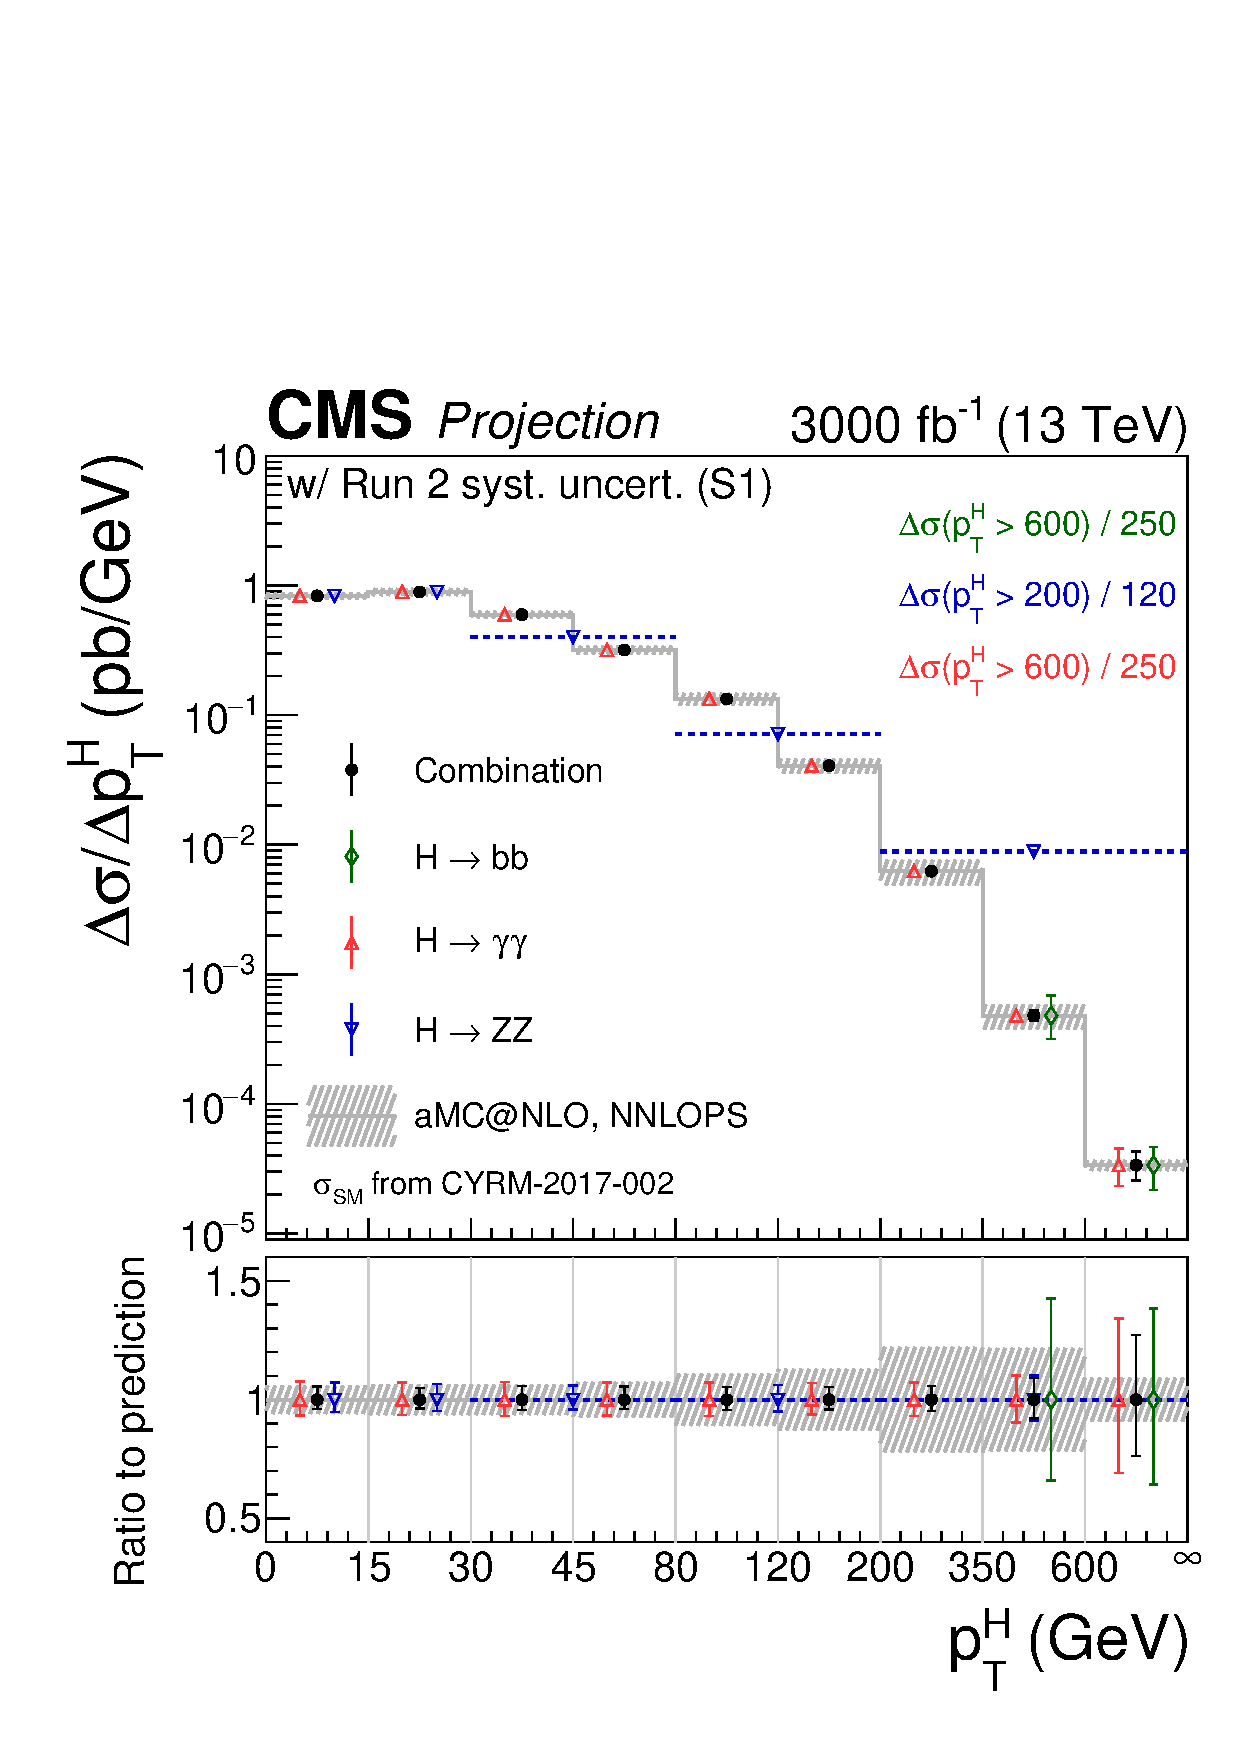
\includegraphics[width=0.49\linewidth]{\main/section2/plots/differentials/projectionspectra_pth_smH.pdf}
    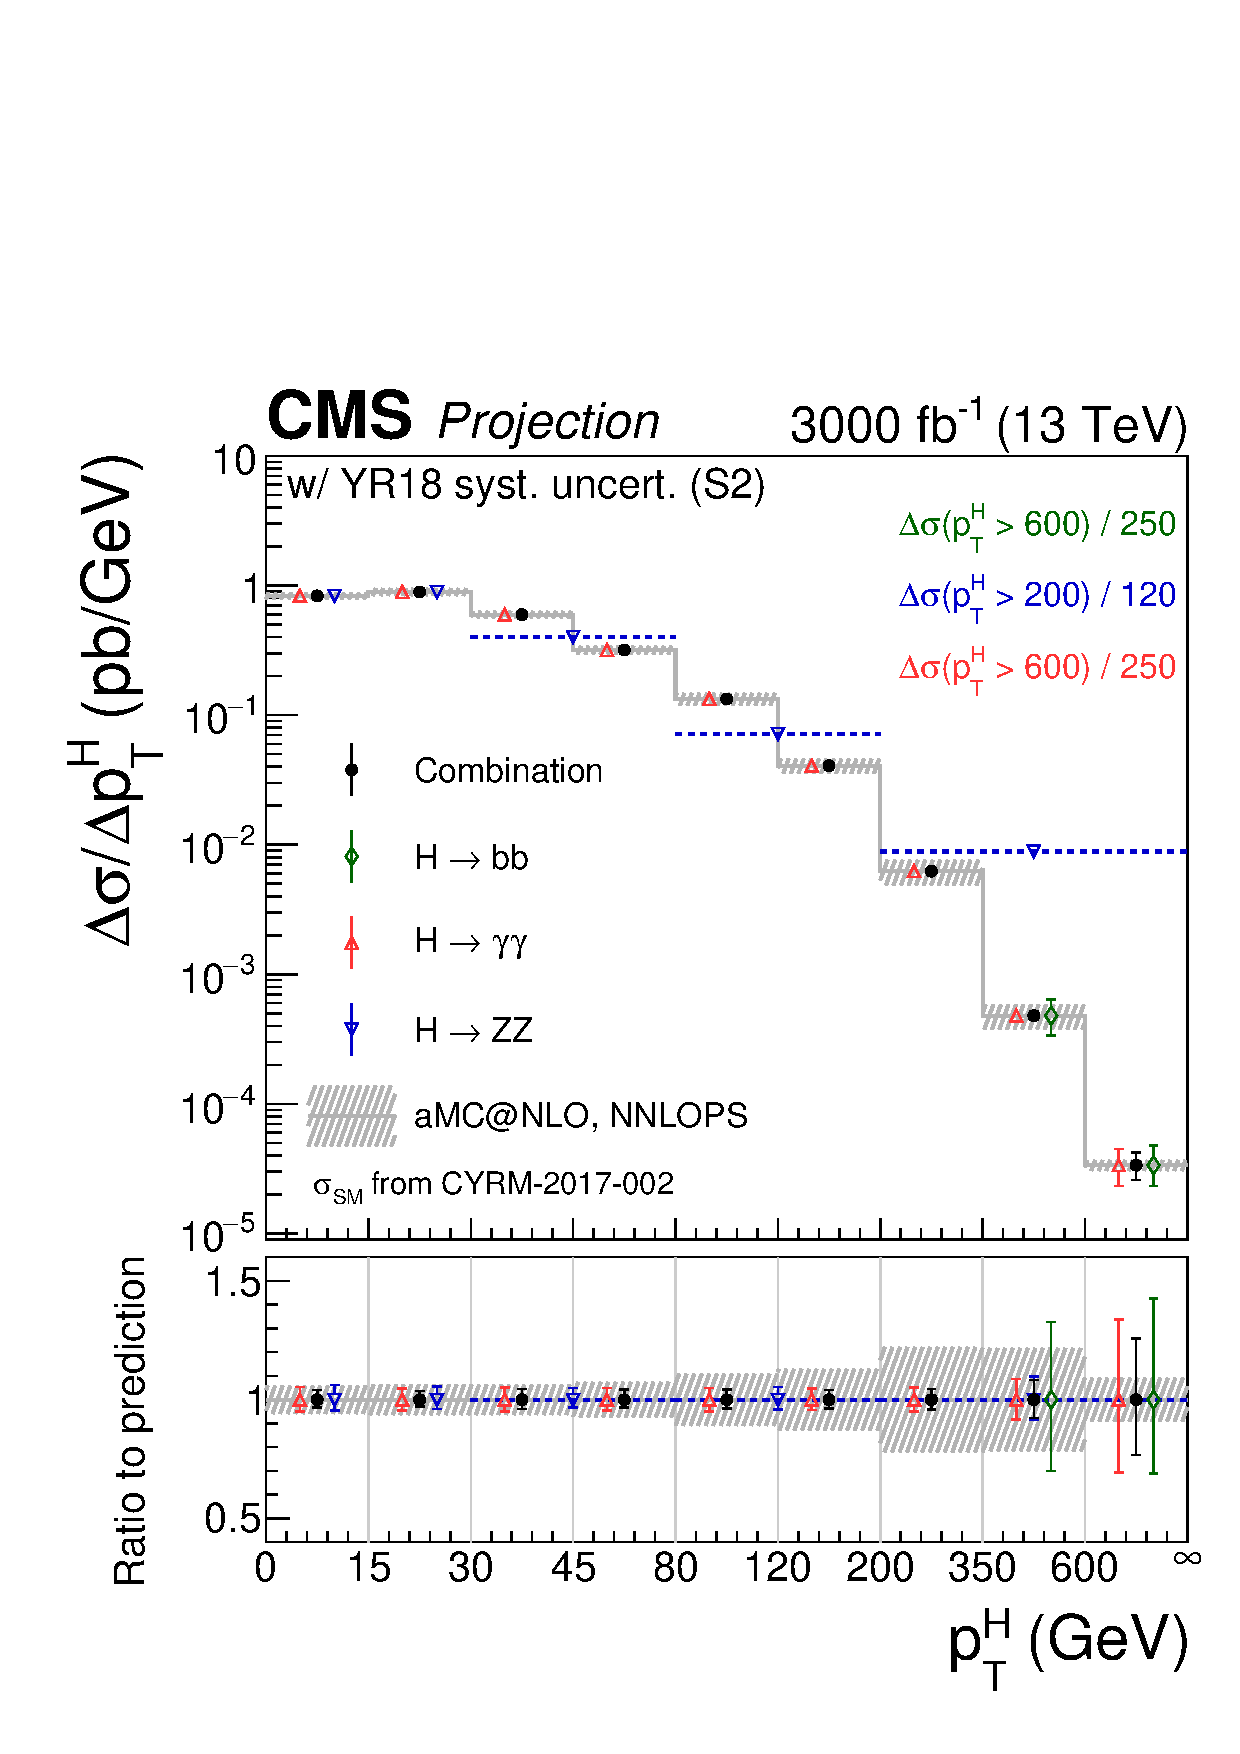
\includegraphics[width=0.49\linewidth]{\main/section2/plots/differentials/projectionspectra_pth_smH_scenario2.pdf}
    \caption{
        Projected differential cross section for $\pTH$ at an integrated luminosity of 3000\fbinv ~\cite{Sirunyan:2018sgc}, under S1 (\UcmsLeft, with Run~2 systematic uncertainties~\cite{CMS-PAS-HIG-17-028}) and S2 (\UcmsRight, with YR18 systematic uncertainties).
        }
    \label{fig:proj_pth}
  \end{center}
\end{figure}

%\begin{table}
%  \footnotesize
%  \centering
%  \begin{tabular}{l|c|c|c|c|c|c|c|c|c}
%    % \hline
%    $\pTH$ (GeV)       & 0-15    &  15-30   &  30-45    &  45-80   &  80-120  &  120-200  &  200-350  &  350-600  &  600-$\infty$  \\
%    \hline
%    $\hgg$       & $7.2\%$ & $6.8\%$ & $7.1\%$ & $6.9\%$            & $7.1\%$ & $6.7\%$            & $7.1\%$ & $9.9\%$  & $32.5\%$ \\ 
%    % \hline 
%    $\hzz$       & $6.2\%$ & $5.7\%$ & \multicolumn{2}{c|}{$5.0\%$} & \multicolumn{2}{c|}{$5.5\%$} & \multicolumn{3}{c}{$9.6\%$} \\ 
%    % \hline 
%    $\hbb$       & \multicolumn{7}{c|}{\textit{None}}                                              & $38.2\%$ & $37.1\%$ \\ 
%    % \hline 
%    Combination  & $4.7\%$ & $4.4\%$ & $5.0\%$ & $4.7\%$            & $4.8\%$ & $4.7\%$            & $5.2\%$ & $8.5\%$  & $25.4\%$ \\
%    % \hline
%  \end{tabular}
%  \caption{Relative uncertainties on the projected $\pTH$ spectrum measurements by ATLAS and CMS under S1 at $3000\fbinv$. {\textbf{The table will be reformatted to include ATLAS' uncertainties}}}
%\label{tab:proj_pth_unc_scen1}
%\end{table}

%\begin{table}
%  \footnotesize
%  \centering
%  \begin{tabular}{l|c|c|c|c|c|c|c|c|c}
%    % \hline
%    $\pTH$ (GeV)       & 0-15    &  15-30   &  30-45    &  45-80   &  80-120  &  120-200  &  200-350  &  350-600  &  600-$\infty$  \\
%    \hline
%    $\hgg$       & $5.1\%$ & $4.6\%$ & $5.1\%$ & $4.8\%$            & $4.9\%$ & $4.5\%$            & $5.1\%$ & $8.6\%$  & $32.2\%$ \\ 
%    % \hline 
%    $\hzz$       & $5.4\%$ & $4.8\%$ & \multicolumn{2}{c|}{$4.1\%$} & \multicolumn{2}{c|}{$4.7\%$} & \multicolumn{3}{c}{$9.1\%$} \\ 
%    % \hline 
%    $\hbb$       & \multicolumn{7}{c|}{\textit{None}}                                              & $31.4\%$ & $36.8\%$ \\ 
%    % \hline 
%    Combination  & $3.7\%$ & $3.3\%$ & $4.2\%$ & $3.7\%$            & $4.0\%$ & $3.8\%$            & $4.4\%$ & $8.0\%$  & $24.5\%$ \\
%    % \hline
%  \end{tabular}
%  \caption{Relative uncertainties on the projected $\pTH$ spectrum measurements by ATLAS and CMS under S2 at $3000\fbinv$. {\textbf{The table will be reformatted to include ATLAS' uncertainties}}}
%  \label{tab:proj_pth_unc_scen2}
%\end{table}


\begin{table}[th]
  %\footnotesize 
  \resizebox{\textwidth}{!}{
  \centering
  \begin{tabular}{l|cccccccc|c|c|c|c|c|c|c|c}
    %% \multicolumn{1}{l}{} & \multicolumn{1}{l}{} & \multicolumn{1}{l}{} & \multicolumn{1}{l}{} & \multicolumn{1}{l}{} & \multicolumn{1}{l}{} & \multicolumn{1}{l}{} & \multicolumn{1}{l}{} & \multicolumn{1}{l}{} & \multicolumn{1}{l}{} & \multicolumn{1}{l}{} & \multicolumn{1}{l}{} & \multicolumn{1}{l}{} & \multicolumn{1}{l}{} & \multicolumn{1}{l}{} & \multicolumn{1}{l}{} & \multicolumn{1}{l}{} \\[\dimexpr-\normalbaselineskip-\arrayrulewidth] % Correct for mis-alignment
    \hline
    \hline
    \multicolumn{17}{c}{3000 fb$^{-1}$ ATLAS}                                                                                                                                                                                                 \\
    \hline
    \hline
    $\pTH$ [\UGeV] & \multicolumn{2}{c|}{0-10}  & \multicolumn{2}{c|}{10-15} & \multicolumn{2}{c|}{15-20} & \multicolumn{2}{c|}{20-30} & 30-45  & 45-60   & 60-80   & 80-120  & 120-200 & 200-350 & \multicolumn{2}{c}{350-1000} \\
    \hline
    $\hgg$       & \multicolumn{2}{c|}{6.5\%} & \multicolumn{4}{c|}{5.9\%} & \multicolumn{2}{c|}{6.2\%} & 6.0\%                      & 6.5\%  & 6.7\%   & 6.0\%   & 5.4\%   & 6.3\%   & \multicolumn{2}{c}{9.5\%}              \\
    \hline
    $\hzz$       & \multicolumn{2}{c|}{9.0\%} & \multicolumn{2}{c|}{8.1\%} & \multicolumn{2}{c|}{8.9\%} & \multicolumn{2}{c|}{6.9\%} & 6.3\%  & 6.8\%   & 6.8\%   & 6.2\%   & 6.7\%   & 13.2\%  & \multicolumn{2}{c}{24.3}     \\
    \hline
    Combination  & \multicolumn{2}{c|}{5.5\%} & \multicolumn{4}{c|}{4.8\%} & \multicolumn{2}{c|}{5.0\%} & 4.7\%                      & 5.0\%  & 5.1\%   & 4.6\%   & 4.4\%   & 5.4\%   & \multicolumn{2}{c}{8.7\%}              \\
    \hline
    \hline
    \multicolumn{17}{c}{3000 fb$^{-1}$ CMS}                                                                                                                                                                                                   \\
    \hline
    \hline
    $\pTH$ [\UGeV] & \multicolumn{4}{c|}{0-15}  & \multicolumn{4}{c|}{15-30} & 30-45                      & \multicolumn{2}{c|}{45-80} & 80-120 & 120-200 & 200-350 & 350-600 & 600-$\infty$                                     \\
    \hline
    $\hgg$       & \multicolumn{4}{c|}{5.1\%} & \multicolumn{4}{c|}{6.8\%} & 7.1\%                      & \multicolumn{2}{c|}{6.9\%} & 7.1\%  & 6.7\%   & 7.1\%   & 9.9\%   & 32.5\%                                           \\     
    \hline
    $\hzz$       & \multicolumn{4}{c|}{5.4\%} & \multicolumn{4}{c|}{5.7\%} & \multicolumn{3}{c|}{5.0\%} & \multicolumn{2}{c|}{5.5\%} & \multicolumn{3}{c}{9.6\%}                                                               \\ 
    \hline
    $\hbb$       & \multicolumn{14}{c|}{none} & 38.2\%                     & 37.1\%                                                                                                                                            \\ 
    \hline
    Combination  & \multicolumn{4}{c|}{4.7\%} & \multicolumn{4}{c|}{4.4\%} & 5.0\%                      & \multicolumn{2}{c|}{4.7\%} & 4.8\%  & 4.7\%   & 5.2\%   & 8.5\%   & 25.4\%                                           \\
    \hline
    \hline
    \multicolumn{17}{c}{6000 fb$^{-1}$}                                                                                                                                                                                                   \\
    \hline
    \hline
    Combination  & \multicolumn{4}{c|}{4.0\%} & \multicolumn{4}{c|}{3.7\%} & 4.0\% & \multicolumn{2}{c|}{3.9\%} & 4.0\% & 4.0\% & 4.3\% & 6.3\% & 18.3\% \\
    \hline
    \hline
  \end{tabular}
  }
  \caption{Relative uncertainties on the projected $\pTH$ spectrum measurements by ATLAS and CMS under S1 at 3000 fb$^{-1}$.  The relative uncertainty of the CMS projection is also given at 6000 fb$^{-1}$ to represent the sensitivity achievable by an eventual ATLAS and CMS combination. }
  \label{tab:proj_pth_unc_scen1}
\end{table}


\begin{table}[th]
  %%\footnotesize  
  \centering
  \resizebox{\textwidth}{!}{
  \begin{tabular}{l|cccccccc|c|c|c|c|c|c|c|c}
    \multicolumn{1}{l}{} & \multicolumn{1}{l}{} & \multicolumn{1}{l}{} & \multicolumn{1}{l}{} & \multicolumn{1}{l}{} & \multicolumn{1}{l}{} & \multicolumn{1}{l}{} & \multicolumn{1}{l}{} & \multicolumn{1}{l}{} & \multicolumn{1}{l}{} & \multicolumn{1}{l}{} & \multicolumn{1}{l}{} & \multicolumn{1}{l}{} & \multicolumn{1}{l}{} & \multicolumn{1}{l}{} \\[\dimexpr-\normalbaselineskip-\arrayrulewidth] % Correct for mis-alignment
    \hline
    \hline
    \multicolumn{17}{c}{3000 fb$^{-1}$ ATLAS}                                                                                                                                                                                                 \\
    \hline
    \hline
    $\pTH$ [\UGeV] & \multicolumn{2}{c|}{0-10}  & \multicolumn{2}{c|}{10-15} & \multicolumn{2}{c|}{15-20} & \multicolumn{2}{c|}{20-30} & 30-45  & 45-60   & 60-80   & 80-120  & 120-200 & 200-350 & \multicolumn{2}{c}{350-1000} \\
    \hline
    $\hgg$       & \multicolumn{2}{c|}{5.3\%} & \multicolumn{4}{c|}{4.6\%} & \multicolumn{2}{c|}{4.9\%} & 4.7\%                      & 5.4\%  & 5.7\%   & 4.9\%   & 4.2\%   & 5.1\%   & \multicolumn{2}{c}{8.7\%}              \\
    \hline
    $\hzz$       & \multicolumn{2}{c|}{8.3\%} & \multicolumn{2}{c|}{7.6\%} & \multicolumn{2}{c|}{8.3\%} & \multicolumn{2}{c|}{6.3\%} & 5.7\%  & 6.2\%   & 6.3\%   & 5.7\%   & 6.4\%   & 13.1\%  & \multicolumn{2}{c}{23.2\%}   \\
    \hline
    Combination  & \multicolumn{2}{c|}{4.5\%} & \multicolumn{4}{c|}{3.8\%} & \multicolumn{2}{c|}{3.9\%} & 3.6\%                      & 4.1\%  & 4.2\%   & 3.7\%   & 3.5\%   & 4.5\%   & \multicolumn{2}{c}{8.2\%}              \\
    \hline
    \hline
    \multicolumn{17}{c}{3000 fb$^{-1}$ CMS}                                                                                                                                                                                                   \\
    \hline
    \hline
    $\pTH$ [\UGeV] & \multicolumn{4}{c|}{0-15}  & \multicolumn{4}{c|}{15-30} & 30-45                      & \multicolumn{2}{c|}{45-80} & 80-120 & 120-200 & 200-350 & 350-600 & 600-$\infty$                                     \\
    \hline
    $\hgg$       & \multicolumn{4}{c|}{5.1\%} & \multicolumn{4}{c|}{4.6\%} & 5.1\%                      & \multicolumn{2}{c|}{4.8\%} & 4.9\%  & 4.5\%   & 5.1\%   & 8.6\%   & 32.2\%                                           \\     
    \hline
    $\hzz$       & \multicolumn{4}{c|}{5.4\%} & \multicolumn{4}{c|}{4.8\%} & \multicolumn{3}{c|}{4.1\%} & \multicolumn{2}{c|}{4.7\%} & \multicolumn{3}{c}{9.1\%}                                                               \\ 
    \hline
    $\hbb$       & \multicolumn{14}{c|}{none} & 31.4\%                     & 36.8\%                                                                                                                                            \\ 
    \hline
    Combination  & \multicolumn{4}{c|}{3.7\%} & \multicolumn{4}{c|}{3.3\%} & 4.2\%                      & \multicolumn{2}{c|}{3.7\%} & 4.0\%  & 3.8\%   & 4.4\%   & 8.0\%   & 24.5\%                                           \\
    \hline
    \hline
    \multicolumn{17}{c}{6000 fb$^{-1}$}                                                                                                                                                                                                   \\
    \hline
    \hline
    Combination  & \multicolumn{4}{c|}{2.9\%} & \multicolumn{4}{c|}{2.6\%} & 3.2\% & \multicolumn{2}{c|}{2.9\%} & 3.0\% & 2.9\% & 3.2\% & 5.8\% & 17.9\% \\
    \hline
    \hline
  \end{tabular}
  }
  \caption{Relative uncertainties on the projected $\pTH$ spectrum measurements by ATLAS and CMS under S2 at 3000 fb$^{-1}$. The relative uncertainty of the CMS projection is also given at 6000 fb$^{-1}$ to represent the sensitivity achievable by an eventual ATLAS and CMS combination.}
  \label{tab:proj_pth_unc_scen2}
\end{table}

\begin{figure}
  \centering
  \subfloat[][]{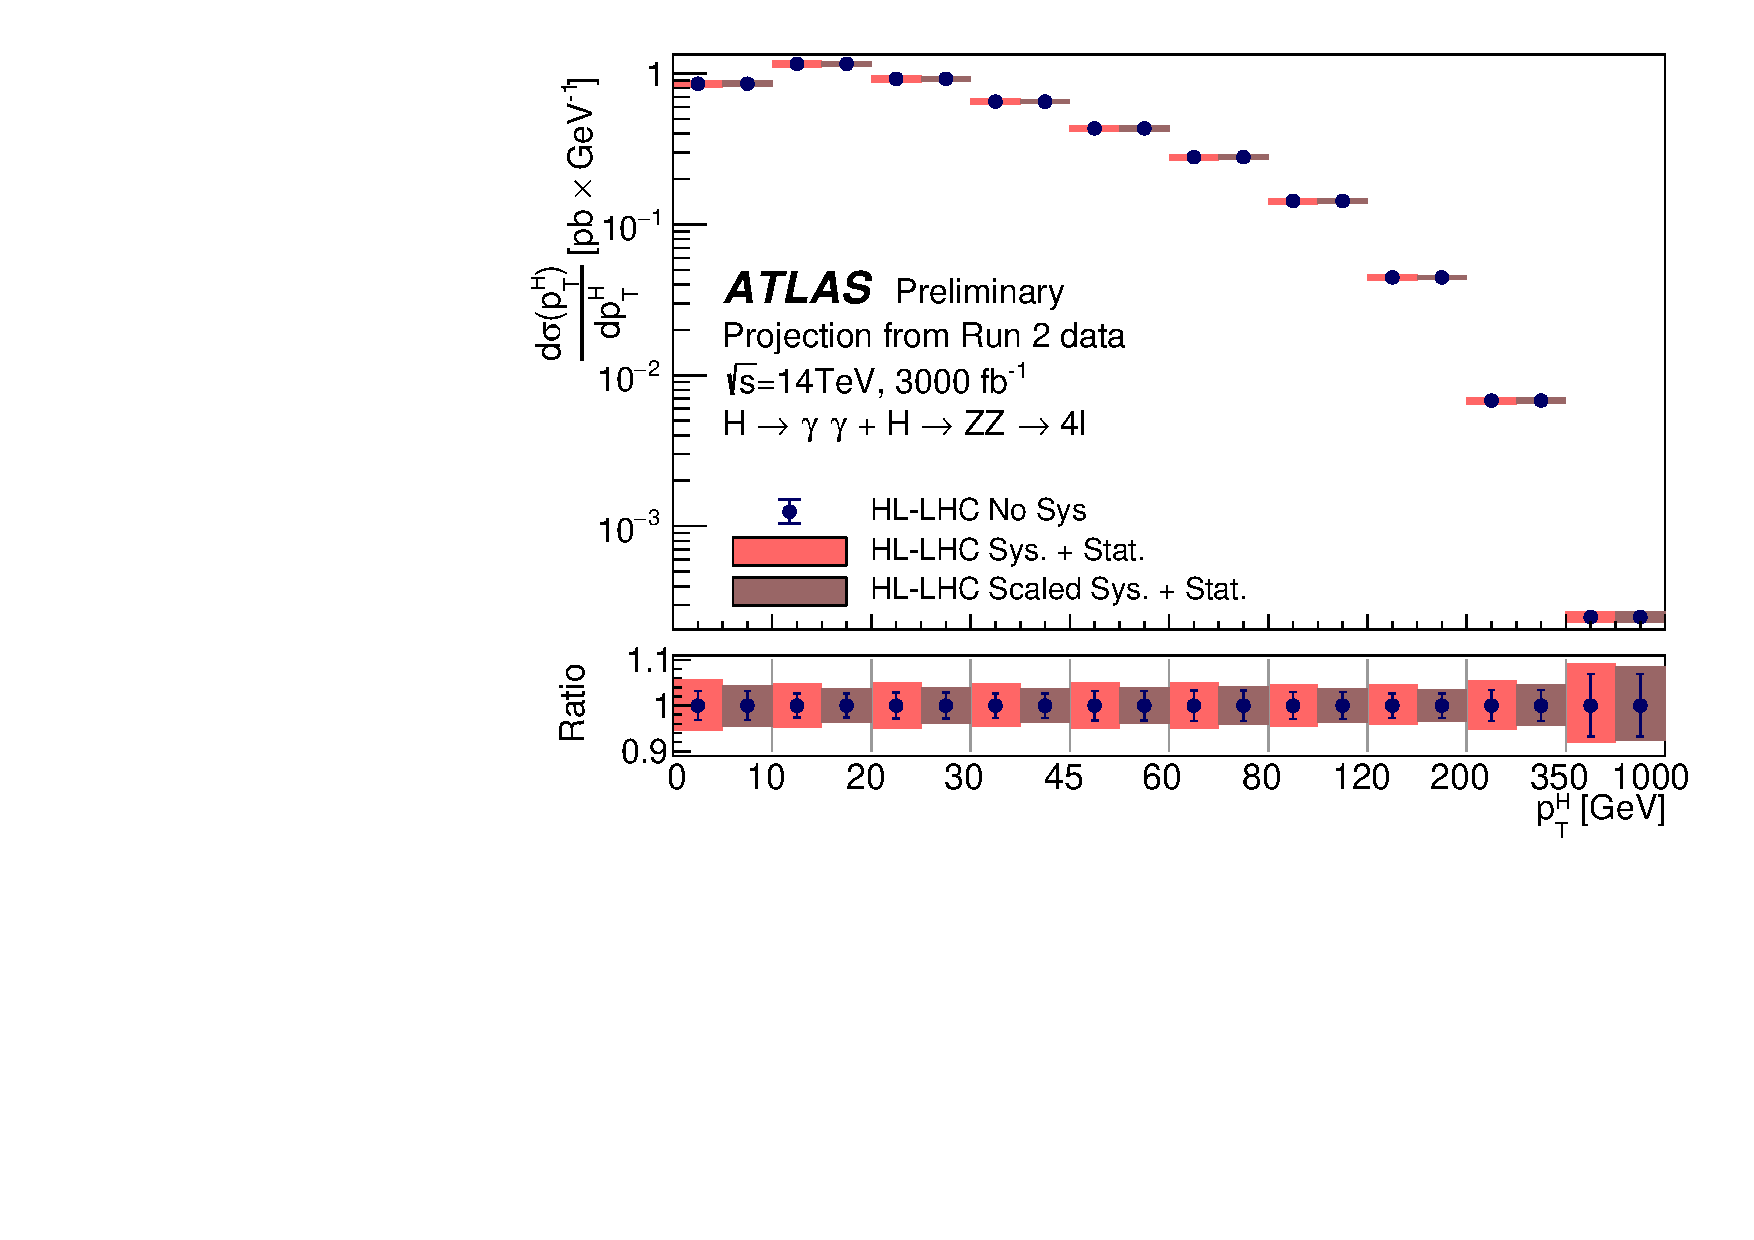
\includegraphics[width=0.48\textwidth]{\main/section2/plots/differentials/ATLAS_hpt_comb}}
  \subfloat[][]{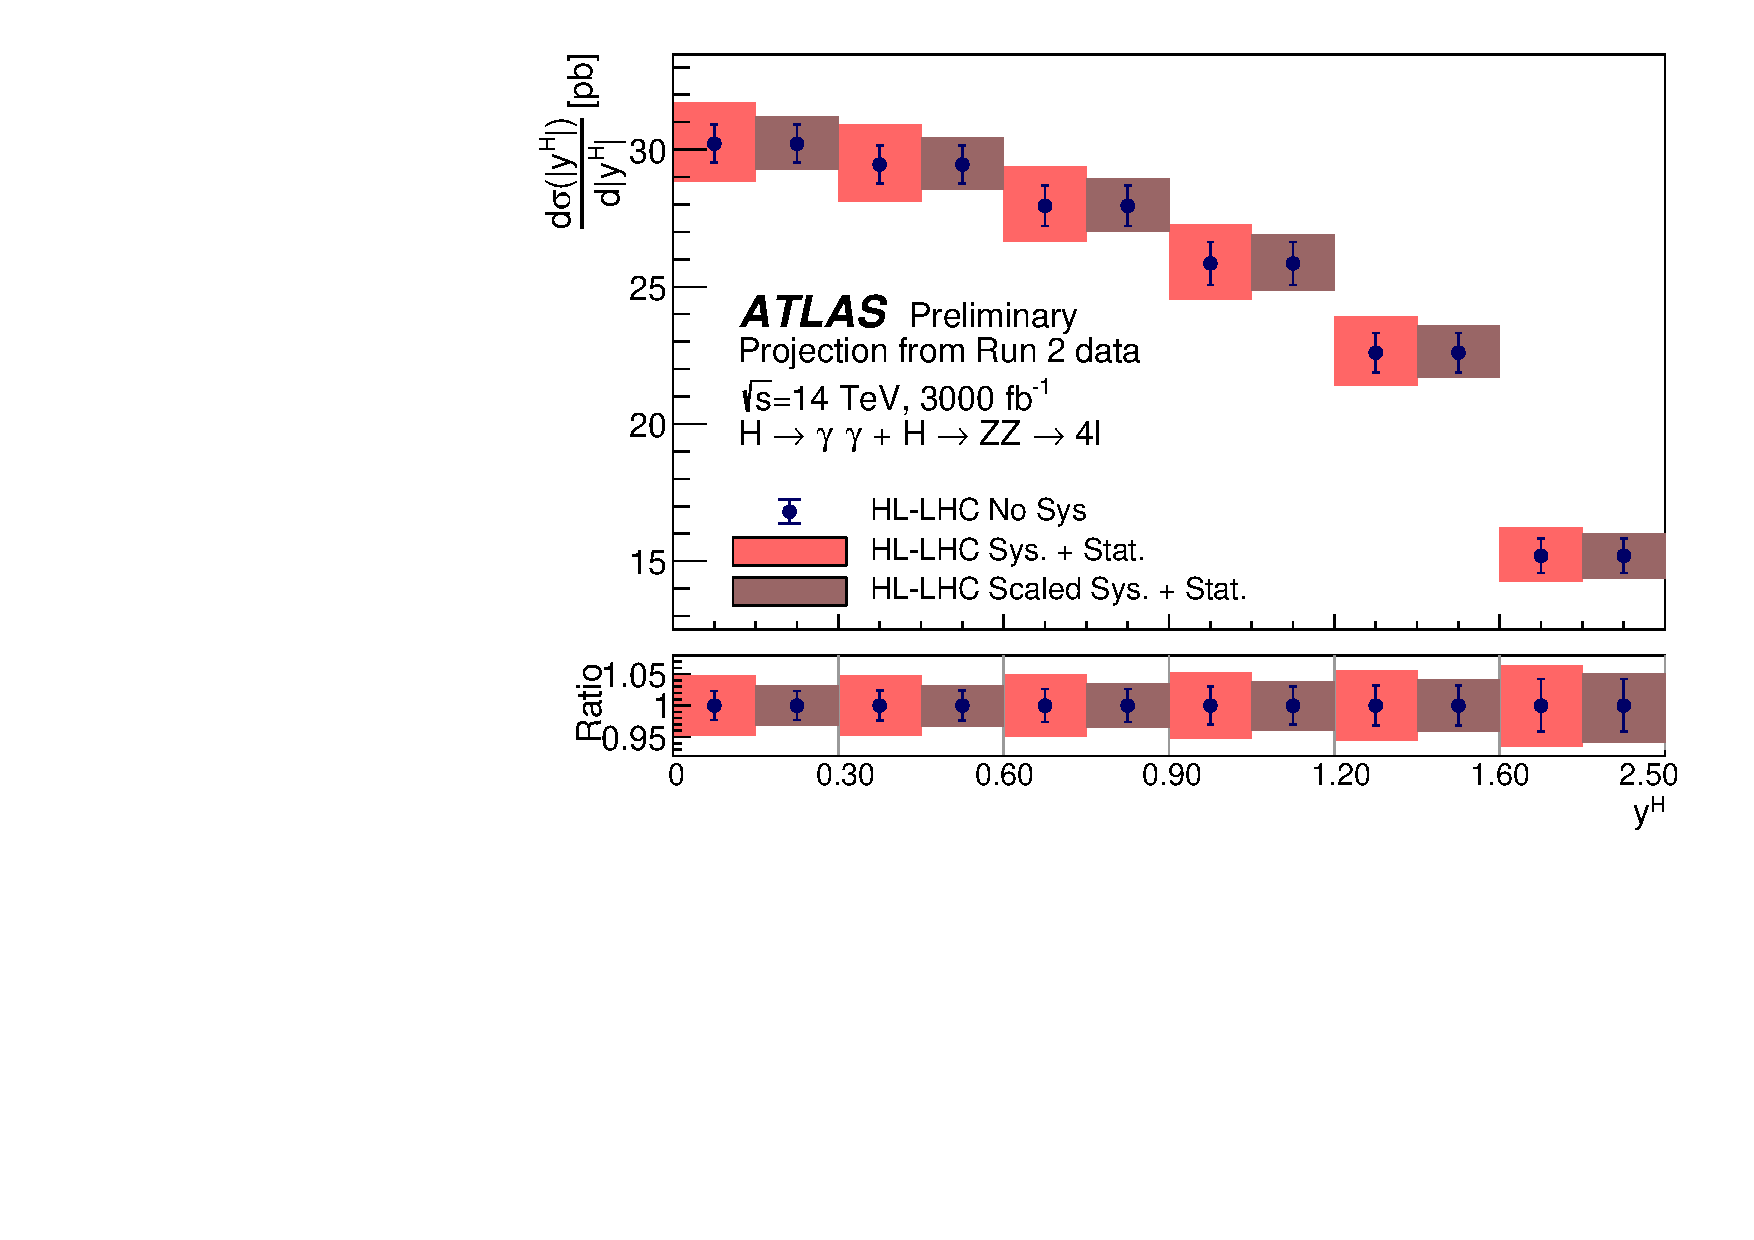
\includegraphics[width=0.48\textwidth]{\main/section2/plots/differentials/ATLAS_y_comb}} \\
  \subfloat[][]{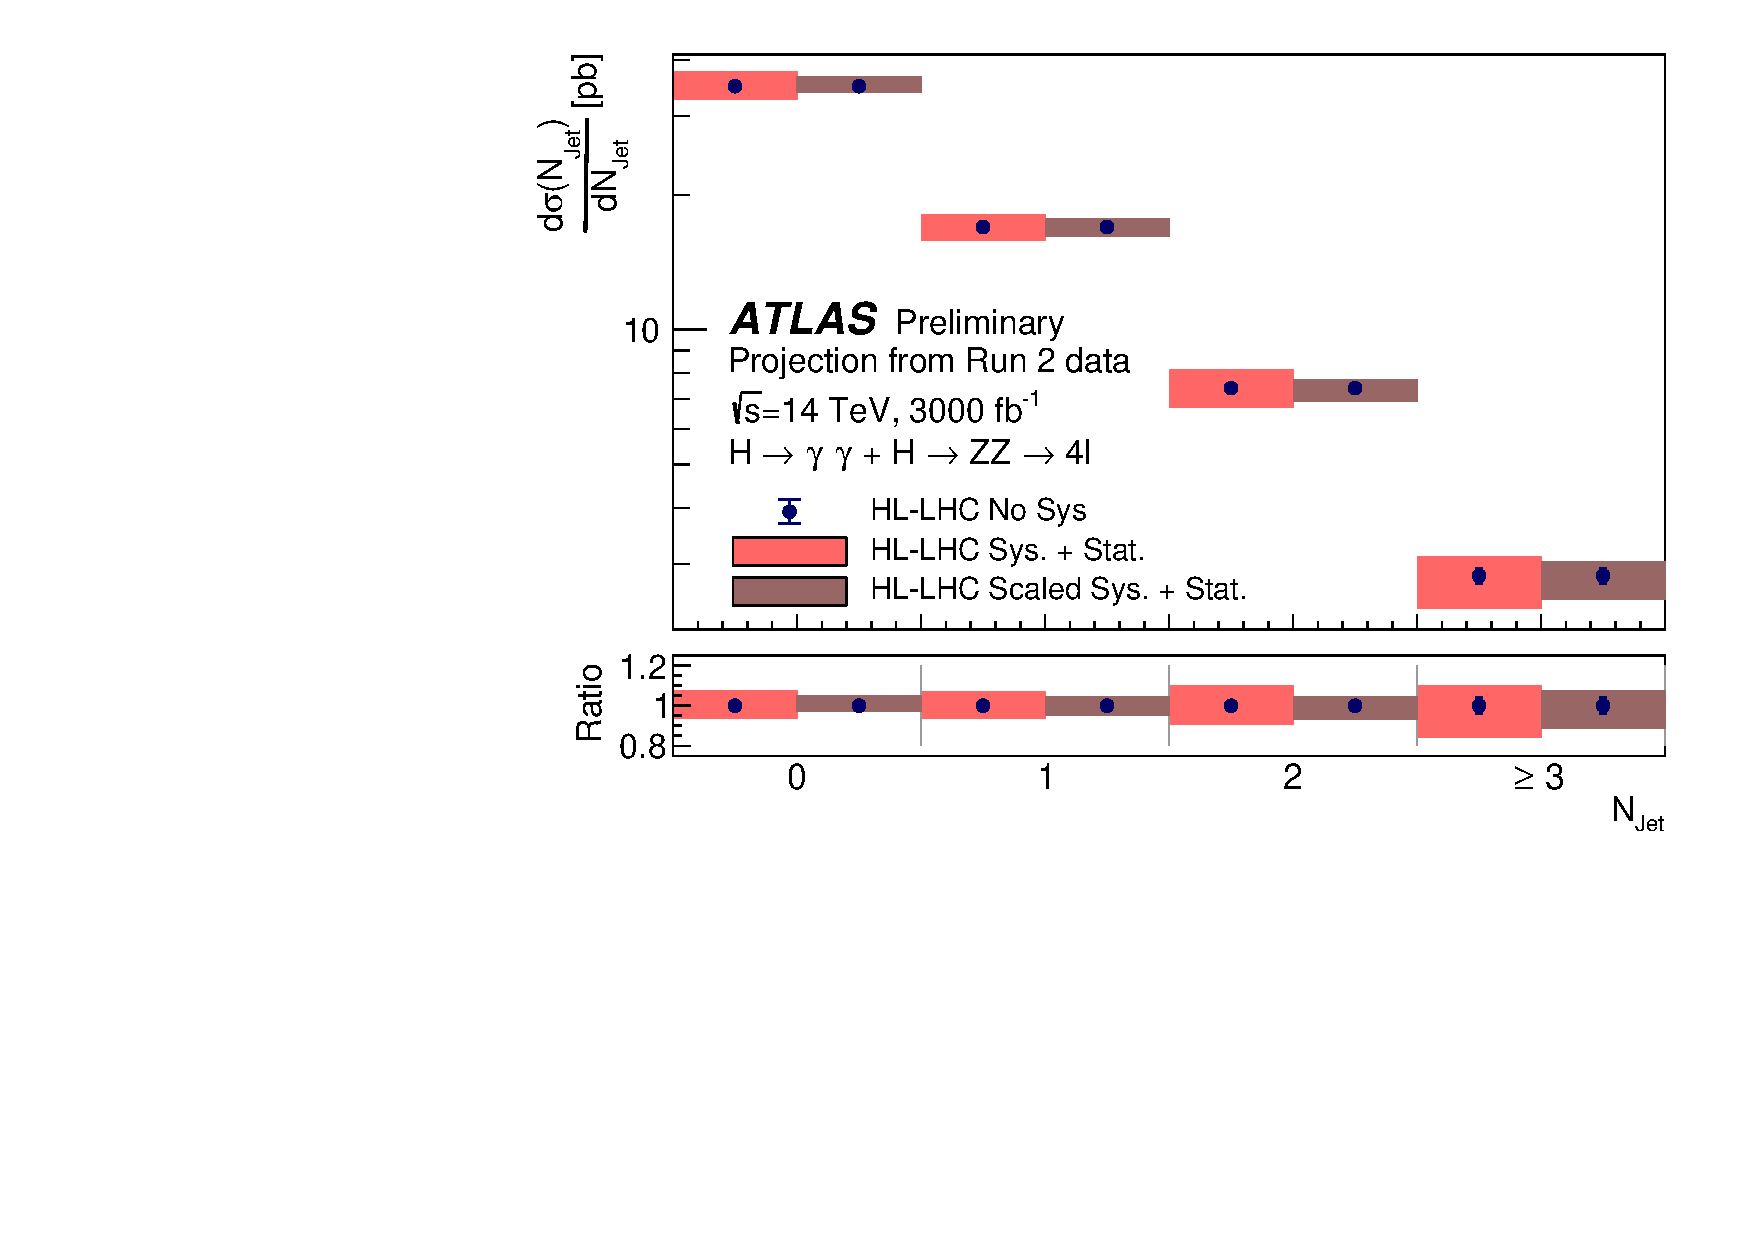
\includegraphics[width=0.48\textwidth]{\main/section2/plots/differentials/ATLAS_njet_comb}}
  \subfloat[][]{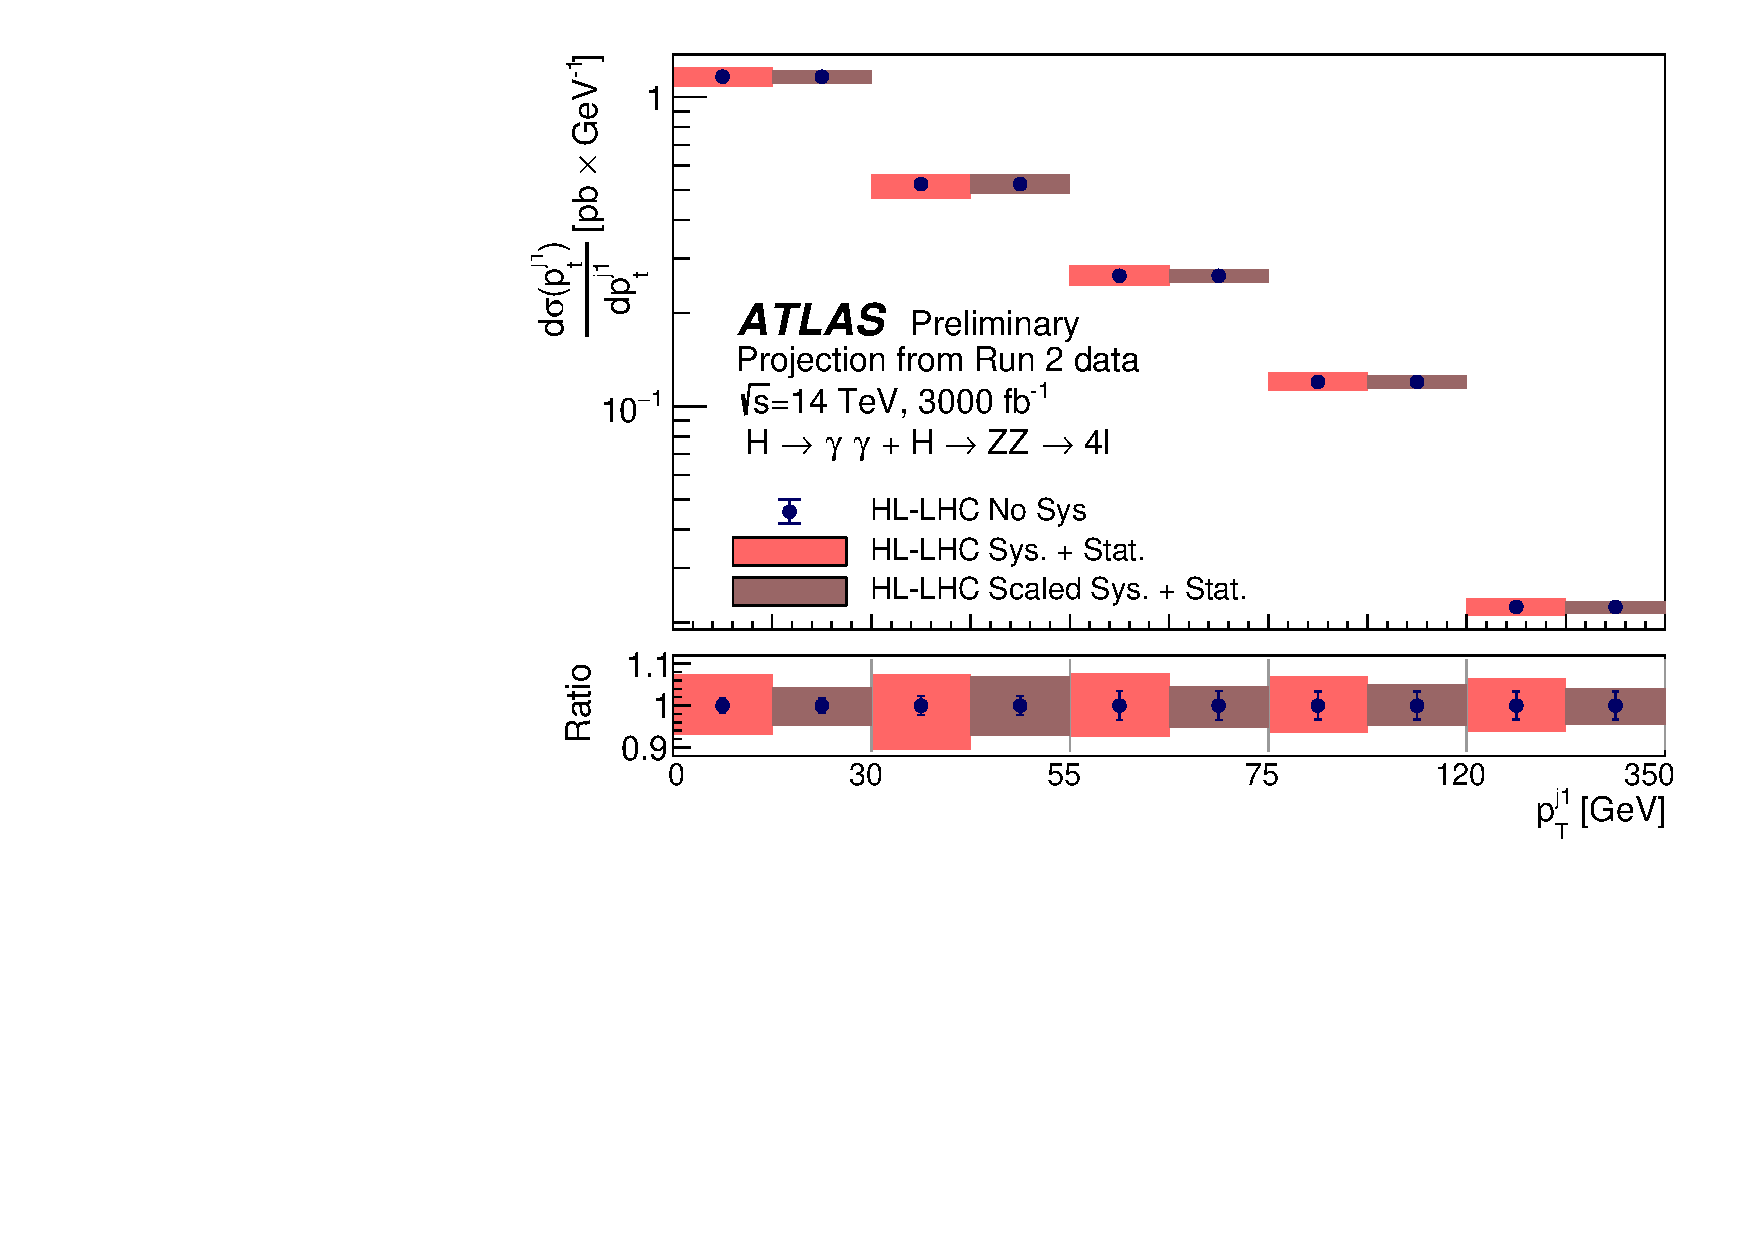
\includegraphics[width=0.48\textwidth]{\main/section2/plots/differentials/ATLAS_ljpt_comb}}
  \caption{Differential cross sections measured by ATLAS in the full phase space, extrapolated to the full HL-LHC luminosity for the combination of the \Hyy\ and \HZZ\ decay channels for (a) Higgs boson transverse momentum $\pTH$, (b) Higgs boson rapidity $|y_H|$, (c) number of jets $N_{\mathrm{jets}}$ with  $p_{\mathrm{T}} >$ 30 \UGeV, and (d) the transverse momentum of the leading $p_{\mathrm{H}}^{j1}$. For each point both the statistical (error bar) and total (shaded area) uncertainties are shown. Two scenarios are shown: one with the current Run2 systematic uncertainty (S1) and one with scaled systematic uncertainties (S2).}
   \label{fig:ATLAS_proj_differential}
\end{figure}

Due to a different choice of $\pTH$ binning by ATLAS and CMS, and the lack of a more sophisticated study of the correlation of systematic uncertainties, it was chosen not to combine the projected spectra presented above. Instead, the projections from CMS are scaled to an integrated luminosity of 6000\fbinv, providing a proxy estimate of the overall sensitivity of an eventual combination of measurements by the two experiments. Figure~\ref{fig:proj_pth_6000} shows the CMS projection at 6000\fbinv, with the same systematic scaling as for the projection at 3000\fbinv.  As expected at very high integrated luminosity, the systematic uncertainties dominate the statistical ones.

\begin{figure}%[hbtp]
  \centering
  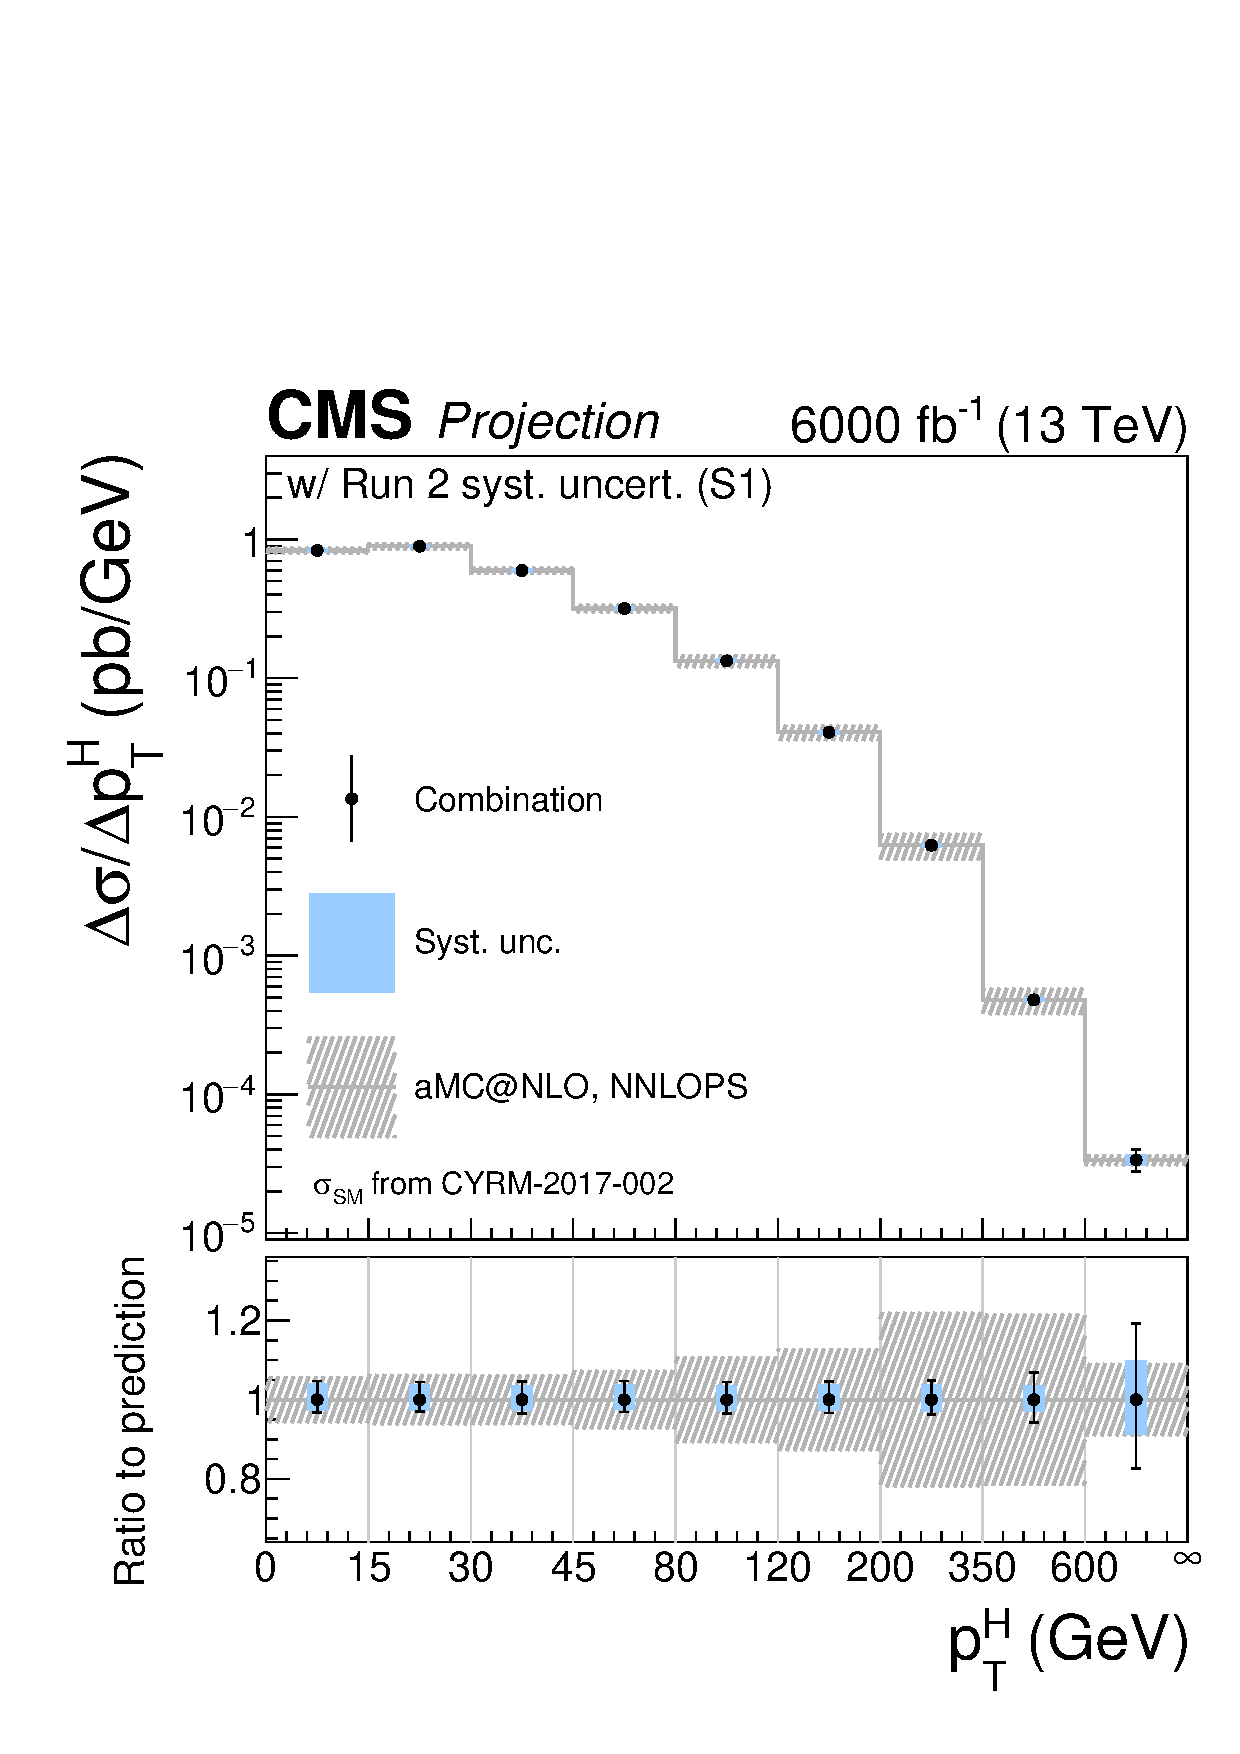
\includegraphics[width=0.49\linewidth]{\main/section2/plots/differentials/projectionspectra_pth_smH_lumi6000.pdf}
  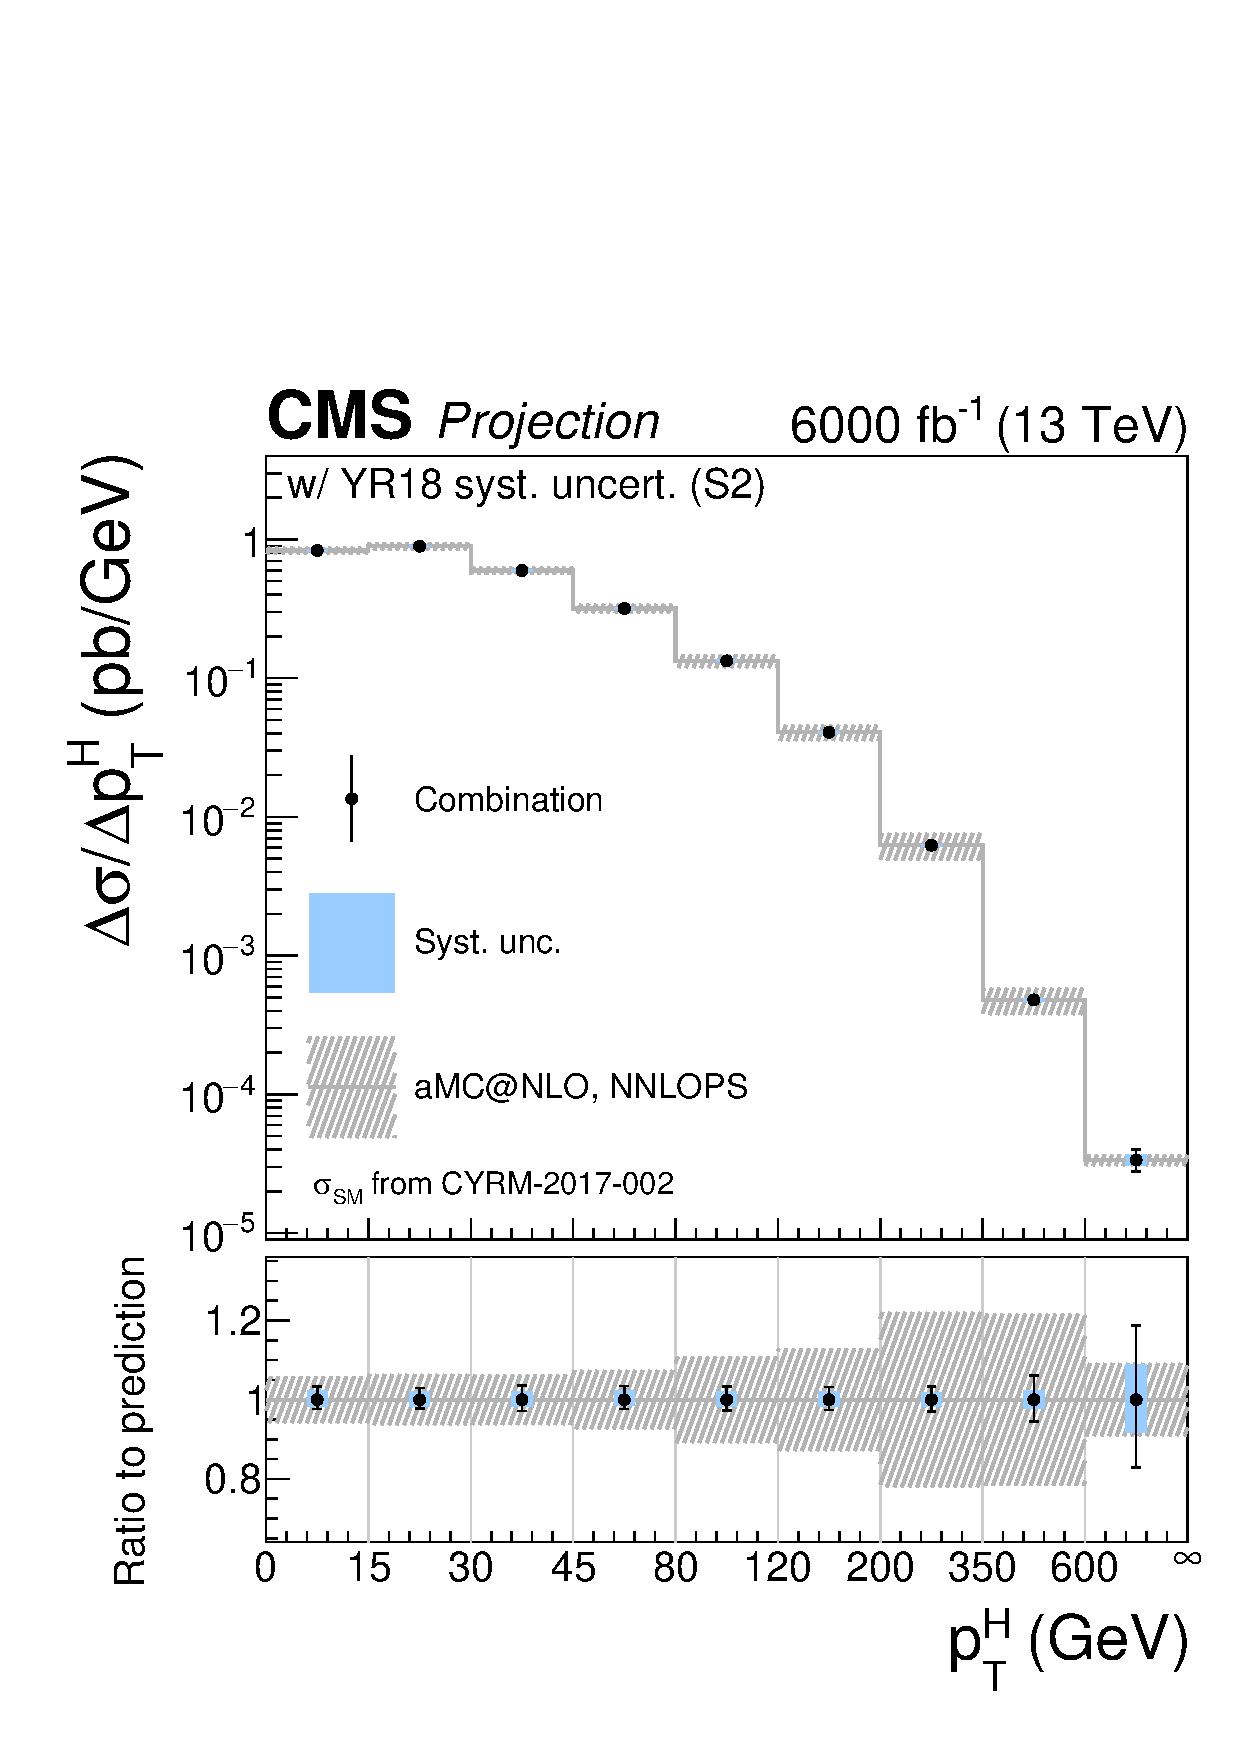
\includegraphics[width=0.49\linewidth]{\main/section2/plots/differentials/projectionspectra_pth_smH_lumi6000_scenario2.pdf}
  \caption{Projected differential cross section for $\pTH$ at an integrated luminosity of 6000\fbinv (representing the sensitivity achievable by an eventual ATLAS and CMS combination), under scenarios S1
    % (\UcmsLeft, with Run~2 systematic uncertainties~\cite{CMS-PAS-HIG-17-028})
    and S2.}
    %(\UcmsRight, with YR18 systematic uncertainties).}
  \label{fig:proj_pth_6000}
\end{figure}

\subsubsection[Measurement of $p_{T}(H)$ spectrum  in \ttH production mode]{Measurement of $p_{T}(H)$ spectrum  in \ttH production mode\footnote{Contact editors: N. Wardle,~J. Langford}}
\label{sec:ttHdiffxs}

This section describes the strategy for measuring the differential $\pt$ cross section for 
Higgs boson production in association with at least one top quark, and decaying to photons ($\ttH+\tH$, $\hgg$), 
at the High-Luminosity LHC with the CMS Phase-2 detector. The $\hgg$ decay mode provides a final state in which the decay of the Higgs boson can be fully reconstructed, and a direct measurement of the $\pt$ differential cross-section can be made. 

The expected precision of the analysis is determined based on simulated proton-proton ($pp$) events, at a centre of mass energy of 14 \UTeV.
Simulated signal and background events are generated using a combination of {\sc POWHEG}
v2.0~\cite{Alioli:2010xd,Nason:2009ai}, {\sc MADGRAPH5\_AMC@NLO} v2.2.2~\cite{Alwall:2014hca}, {\sc SHERPA} v2.2.5~\cite{Gleisberg:2008ta}, and interfaced with {\sc PYTHIA} v8.205~\cite{Sjostrand:2007gs}. The signal and background events are processed with {\sc DELPHES}~\cite{deFavereau:2013fsa}, using the CMS Phase-2 card, to simulate the response of the upgraded CMS detector to showered particles. Full details of the analysis can be found in Ref.~\cite{CMS-PAS-FTR-18-020}.

\subsubsubsection{Analysis strategy}

An event selection is applied to the simulated background and signal events following a similar strategy to the CMS Run 2 $\hgg$ strategy \cite{Sirunyan:2018ouh}. The events are required to contain two photons, with $|\eta^\gamma|$~$<$~2.4 excluding the region 1.44~$<$~$|\eta^\gamma|$~$<$~1.57, with an invariant mass satisfying 100~$<$~$m_{\gamma\gamma}$~$<$~180~\UGeV, where the leading-$\pt$ (sub-leading-$\pt$) photon satisfies $\pt^{\gamma}/m_{\gamma\gamma}$~$>$~1/3 (1/4). The two photons are also required to be separated by $\Delta R_{\gamma\gamma}$~$>$~0.4. The photons must also be isolated, which is achieved by requiring that the sum of charged transverse momentum in a cone of radius $\Delta R_{\gamma}$~=~0.4, centred on the photon direction, is less than 0.3$\, \pt^\gamma$. For events where more than one photon pair passes the selection, then the pair with $m_{\gamma\gamma}$ closest to the Higgs boson mass is chosen.

In order to isolate the production of the Higgs boson in association with top quarks, the selection requires all events to have at least one $b-$tagged jet. Such events are separated into two orthogonal categories based on the decay products of the top quark, a hadronic category and a leptonic category. In the hadronic category, events must contain at least 3 jets, clustered using the anti-$k_{T}$ algorithm with a cone size of 0.4, separated by $\Delta R$~$>$~0.4 with respect to both photon candidates. The jets are required to have $\pt>25$ \UGeV and $|\eta|$~$<$~4. In the leptonic category, only 2 jets are required, however, in addition, the events must contain at  least one isolated muon or electron. The muons or electrons must satisfy $\pt$~$>$~20~\UGeV and $|\eta|$~$<$~2.4, excluding the region 1.44~$<$~$|\eta^\gamma|$~$<$~1.57 for electrons. The muons must satisfy an isolation requirement that the sum of all reconstructed particles $\pt$, inside a cone of radius $\Delta R=0.4$, excluding the muon itself, is less than 0.25 times the transverse momentum of the muon. In addition, for electrons, the invariant mass of pairs formed from the electron and either selected photon, $m_{e\gamma}$, is required to be greater than 95 \UGeV to reduce contamination from $Z\rightarrow e^{+}e^{-}$ decays. Events passing the leptonic category selection are excluded from the hadronic selection to maintain orthogonality of the two categories.  
For the signal extraction, boosted decision tree (BDT) classifiers are trained independently in each channel, which distinguish between signal-like and background-like events, using input variables related to the kinematics of the events, such as the lepton and jet momenta and pseudo-rapidities, and the scalar sum of transverse momentum of all final state objects in the event. Events are required to have output BDT values greater than fixed thresholds, which are tuned to provide the best sensitivity to $\kappa_{\lambda}$. The hadronic category is further split into two different regions of BDT output, for events with di-photon transverse momentum ($\pt^{\gamma\gamma}$) less than 350 \UGeV, to reduce the contamination of gluon fusion Higgs boson production. 

Finally, the events are further divided into six bins of $\pt^{\gamma\gamma}$, given in Tab.~\ref{tab:ttHdiff_CMS_ptbins}, making a total of 17 categories. 

\begin{table}[h]

 \centering
 \begin{tabular}{c|c|c|c|c|c|c}
 %{P{1cm}P{1cm}P{1cm}P{1cm}P{1cm}P{1cm}P{1cm}}
    \hline
    \hline
    \multicolumn{7}{c}{$\pt^{H}$ or $\pt^{\gamma\gamma}$ bin boundaries (\UGeV)}  \\ \hline
    0 & 45 & 80 & 120 & 200 & 350 & $\infty$ \\
    \hline
    \hline
\end{tabular}
\caption{bin boundaries which define the $\pTH$ regions for which the differential cross sections are measured. These also correspond to the bins in which the hadronic and leptonic event categories are sub-divided.}
\label{tab:ttHdiff_CMS_ptbins}
\end{table}

Experimental systematic uncertainties are included in the signal model, which can cause migration both between the different categories and in and out of the fiducial region. The dominant uncertainties are related to the reconstruction and identification efficiencies for photons and b jets as well as the energy scale and resolution of reconstructed jets. 
Furthermore, theoretical uncertainties are included on the rates of $\ggh$ and $\vh$ contamination, which modify both the overall normalisation and the relative contamination between the different categories for these processes. The background estimation follows the same strategy as in the CMS Run 2 $\hgg$ analysis~\cite{Sirunyan:2018ouh}, in that the parameters of the background functions are free to float in the fit, and constrained directly from the data. Therefore the uncertainties on the background will be statistical in nature.
However, the impact of increasing the rate of fake photons in the background component has been studied and was found to reduce the sensitivity to $\kappa_\lambda$ by roughly 10\% in the worst case scenario~\cite{CMS-PAS-FTR-18-020}.  

\subsubsubsection{Differential cross-section results}

In order to account for resolution effects, the signal events are separated based on the $\pt^H$ at generator level.   Signal and background models are constructed using the simulated events in each category. The signal model accounts for the relative populations of events from the different production processes as well as from different $\pTH$ bins, and the di-photon mass resolution expected from events in each category. The background model is constructed from a fit of smoothly falling functions to the weighted sum of simulated background samples, accounting for the different fake photon rates for each source of background and normalised to the  total background yield expected in 3000 fb$^-1$ of High-Luminosity LHC data. The differential cross-section is determined from a simultaneous maximum likelihood fit to an Asimov data set~\cite{Cowan:2010js} corresponding to $3\abinv$, and assuming SM Higgs boson  production in each category.  Systematic uncertainties are accounted for through the introduction of constrained nuisance parameters in the log-likelihood, which are profiled. 

The results of this fit are given in figure~\ref{fig:ttHdiff_CMS_ptH_xs}. The results shown are unfolded back to a fiducial region which is common to both the hadronic and leptonic selections, and shown using only the hadronic or leptonic categories, and their combination. The theoretical uncertainties displayed on the predicted $\ttH+\tH$ cross section are calculated by modifying the renormalisation and factorisation scales up and down by a factor of 2.

\begin{figure}[htb!]
        \centering
        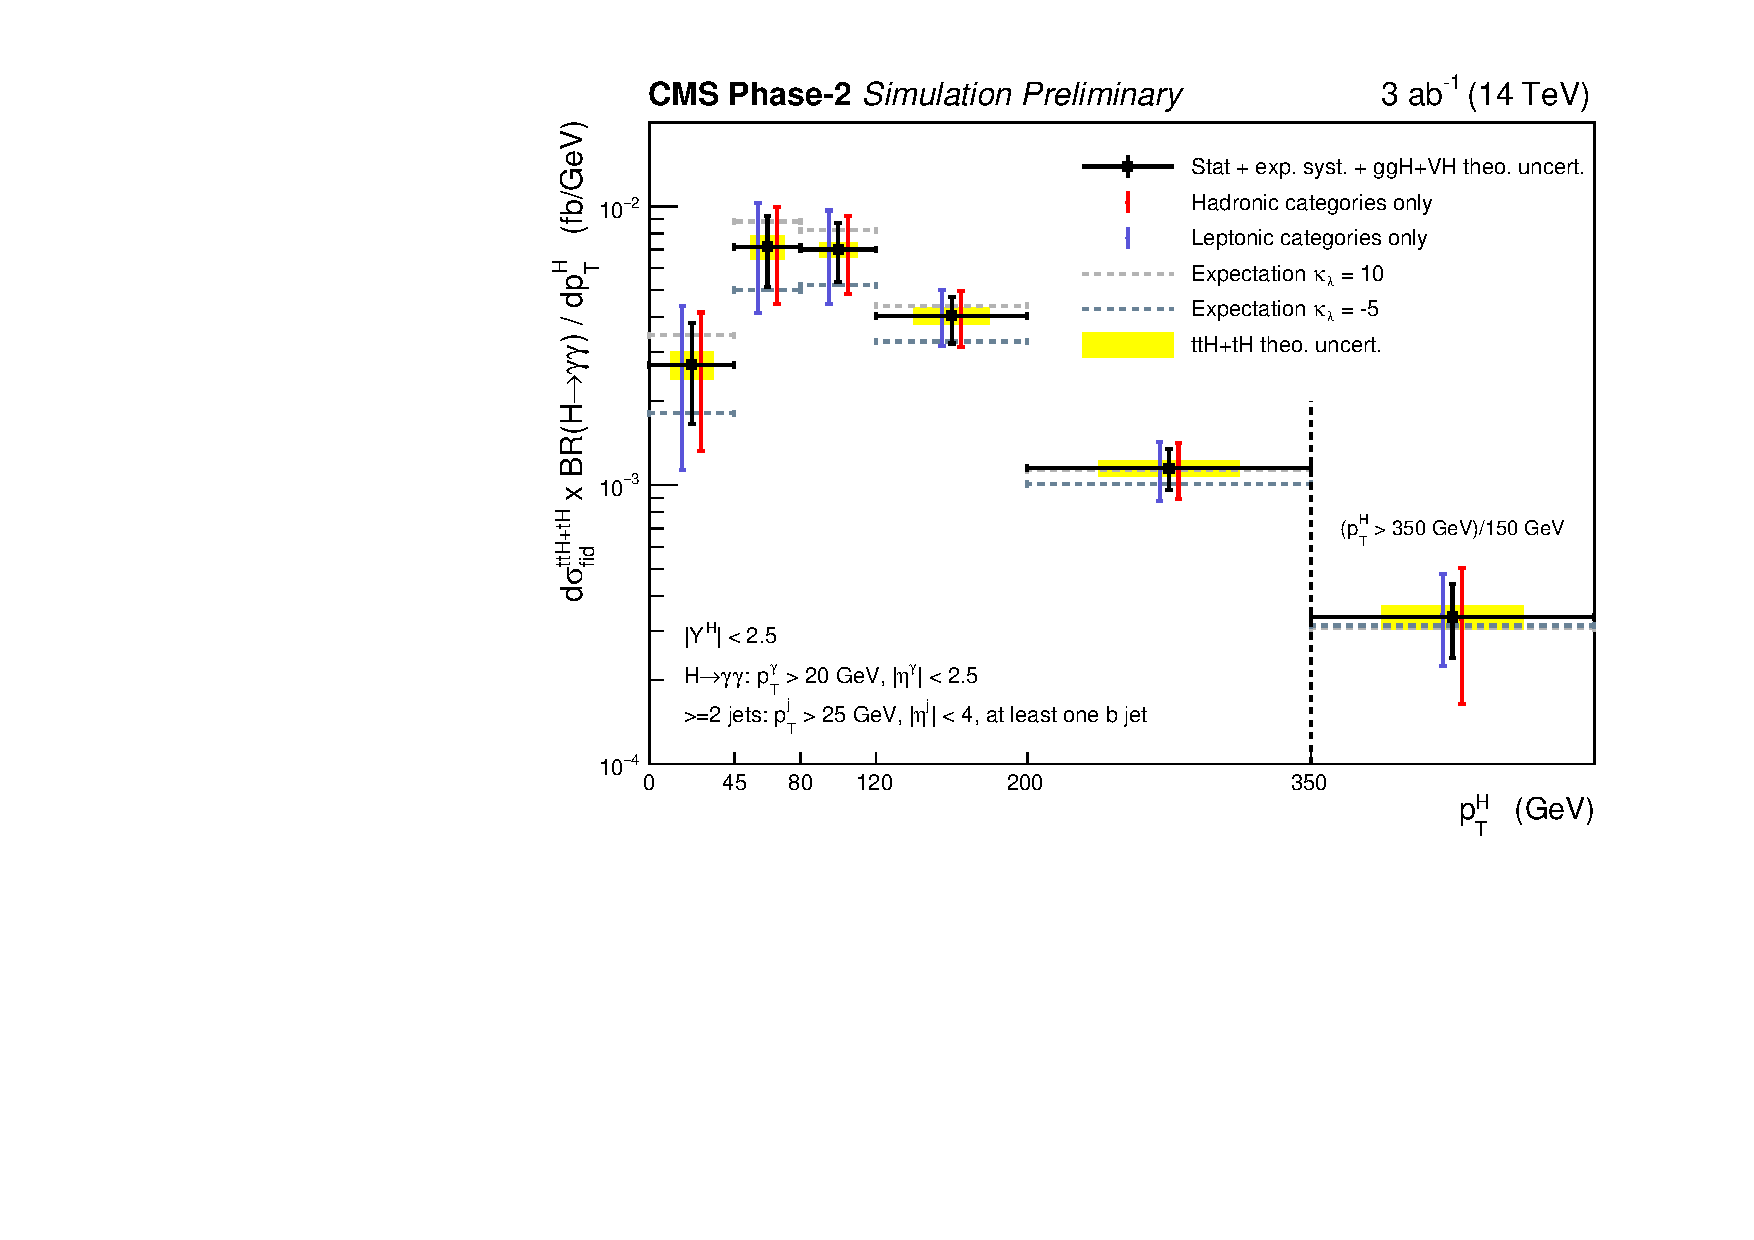
\includegraphics[width=0.6\textwidth]{\main/section2/plots/dXS_dpTH.pdf}
        \caption{The expected $\pt^H$ differential $\ttH$~+~$\tH$ cross sections times branching ratio, along with their uncertainties ~\cite{CMS-PAS-FTR-18-020}. The error bars on the black points include the statistical uncertainty, the experimental systematic uncertainties and the theoretical uncertainties related to the $\ggh$ and $\vh$ contamination, which is subtracted in the fit.  The cross section for $\pTH > 350$ \UGeV is scaled by the width of the previous bin. The expected $\ttH$~+~$\tH$ cross sections for anomalous values of the Higgs boson self-coupling ($\kappa_\lambda$~=~10 and $\kappa_\lambda$~=~-5) are shown by the horizontal dashed lines.}
        \label{fig:ttHdiff_CMS_ptH_xs}
\end{figure}

